\documentclass[11pt]{article}
    \usepackage{amsmath}
    \usepackage[pdftex]{graphicx}
    %\usepackage[usenames,dvipsnames,svgnames,table]{xcolor}
    \usepackage{amsmath,amsthm,amssymb,color,wrapfig,floatflt,amsfonts,listings,fancyhdr}
    \usepackage[parfill]{parskip}
    %\pagestyle{plain}
    \setlength\topmargin{.1cm}
    %\setlength\textheight{8in}
    \setlength\oddsidemargin{.1in}
    \setlength\evensidemargin{.1in}
    \setlength\textwidth{6.51in}
    %\setlength\headheight{52.5pt}
    \usepackage{fancyhdr}
    \usepackage[algosection, boxruled, linesnumbered]{algorithm2e}
    \pagestyle{fancy}
    \lhead{Arvind Ramaswami}
    \rhead{HW3}
    \chead{CS 4641 Machine Learning}
    \lfoot{}
    \cfoot{Page {\thepage}}
    \rfoot{}
    \newcommand{\RR}{\mathbb{R}}
    \newcommand{\CC}{\mathbb{C}}
    \newcommand{\HH}{\mathbb{H}}
    \newcommand{\BB}{\mathbb{B}}
    \newcommand{\ZZ}{\mathbb{Z}}
    \newcommand{\QQ}{\mathbb{Q}}
    \newcommand{\NN}{\mathbb{N}}
    \newcommand{\cP}{\mathcal{P}}
    \renewcommand{\And}{\wedge}
    \newcommand{\Or}{\vee}
    \newcommand{\Implies}{\Rightarrow}
    \newcommand{\Not}{\sim}
    \begin{document}
        \section{Introduction}
            
            This project investigates algorithms in unsupervised
            learning: PCA (Principal Component Analysis), K-means
            clustering and GMMs (Gaussian Mixture Models).

            \subsection{Experiments}
            
            First, two datasets are chosen. In this experiment, the datasets are the Mushrooms
            dataset from Kaggle and the Pima Indians Diabetes dataset from Kaggle.

            Then, two clustering algorithms (K-means clustering and GMMs via expectation maximization)
            are run.

            Then, the datasets are reduced into fewer dimensions using Principal Component Analysis.
            The clustering algorithms are re-performed on the reduced dataset.

            Then, the original results of the PCA algorithm on the Pima Indians
            Diabetes dataset are taken, and the neural network is trained on this reduced
            dataset. To evaluate the accuracy of the neural network, both the training
            and testing datasets are projected with the dimensionality function that had been generated
            before.


            Finally, the training dataset of the Pima Indians
            Diabetes dataset is clustered using the k-Means and GMM algorithms
            and reduced to fewer dimensions using the two algorithms. In these specific experiements, the k-Means
            algorithm reduces the data to the cluster-distance space (sklearn's \texttt{transform}
            function), while the GMM reduces each datapoint to the probabilities
            of the datapoint being in each cluster (sklearn's \texttt{predict\char`_proba} function).
            Then, with the clustering algorithms used on the training set,
            the test set is also reduced to those same features. A neural network
            is then trained on the training datasets produced by the two clustering
            algorithms.
           
        \section{Results}

            \subsection{Initial clustering}


%                 Given enough data points, it is possible to make quantitative measurements to
%                 extrapolate how much information the clustering algorithm can give about the
%                 structure of the true labels.

%                 For each cluster number, if the number of occurrences of that number for data points
%                 for every label is about the same, then that cluster does not give much information about
%                 what separates the data. However, if a cluster prefers one class label over the other class
%                 labels, it does give a great insight about the structure of the labels.

%                 There are some slight patterns that can be seen by running the clustering algorithms
%                 on the raw datasets (but these patterns do not give much insight on how the
%                 labels themselves are distributed).

%                 Here are the results of the cluster categorizations that were produced when running either algorithm
%                 for this dataset (the cluster categories of the first 200 elements of the training set
%                 are shown, with a parameter such that the number of clusters is equal to 10):

                
%                 [8 7 0 1 7 7 4 3 7 1 4 6 6 7 4 4 3 7 6 0 0 6 9 3 7 8 7 6 1 9 3 1 7 7 1 4 6
%  3 7 0 9 6 1 6 7 1 1 0 6 4 7 1 0 6 6 1 1 7 0 9 9 7 0 7 6 7 3 7 1 9 4 1 4 0
%  6 7 7 5 5 4 1 6 6 6 0 1 0 0 6 3 9 7 1 0 6 0 5 1 4 7 3 4 4 7 5 1 6 7 6 4 6
%  7 7 6 0 1 1 9 4 6 6 0 6 4 1 7 4 1 4 1 3 3 1 6 7 7 7 4 7 7 7 6 7 7 3 0 7 1
%  8 9 0 4 7 7 3 6 6 1 9 0 0 5 4 6 7 1 4 6 0 0 6 7 9 9 0 4 7 3 9 4 0 4 1 6 6
%  6 9 7 3 1 3 6 6 8 1 6 7 7 4 3] (K-means)

%                 [5 1 1 3 1 1 1 3 1 6 1 3 3 1 1 1 6 1 6 1 1 3 4 0 1 5 1 3 0 4 3 6 1 1 6 1 3
%  3 1 1 4 3 3 3 1 6 6 1 3 8 1 6 1 3 3 6 6 1 3 4 4 1 1 1 3 1 3 1 3 4 1 3 1 6
%  6 1 1 2 2 1 6 3 3 3 3 3 1 1 6 6 4 1 3 1 6 1 2 0 8 1 4 1 1 1 2 6 3 1 6 1 3
%  1 1 3 1 6 0 4 1 6 3 1 3 8 6 1 1 6 1 6 3 0 3 6 1 1 1 1 1 1 1 6 1 1 3 1 1 6
%  3 4 1 1 1 1 3 3 3 6 4 1 1 4 1 6 1 6 1 6 9 1 3 1 4 4 3 1 1 3 4 1 1 1 3 3 3
%  3 4 1 6 3 0 3 3 5 6 3 1 1 6 0] (GMM)

%                 As a reference, here are the first 200 training labels:

%                 [0 0 0 0 1 0 1 0 1 1 1 1 0 0 1 1 1 0 0 0 0 1 0 0
%   1 0 0 0 1 1 0 1 0 0 0 0 0 0 1 0 0 0 0 0 0 0 1 0
%   0 1 1 0 0 0 0 1 1 0 0 0 0 0 0 1 0 1 0 0 0 0 0 0
%   0 0 0 0 0 0 1 0 1 0 0 0 0 0 0 0 0 1 1 0 0 0 0 0
%   0 0 1 1 0 1 1 1 1 1 0 0 0 1 0 0 1 0 0 1 1 0 1 0
%   0 0 0 1 0 1 0 0 1 0 0 1 0 0 0 0 1 1 1 0 0 0 1 0
%   0 0 0 0 0 0 0 1 0 0 0 0 0 1 0 0 0 0 0 0 0 1 0 0
%   1 0 0 0 0 1 0 1 0 1 0 1 0 0 0 0 0 1 1 0 1 0 1 0
%   0 1 1 0 0 1 1 1]

%                 When comparing the results of K-means and GMMs side by side, we can see
%                 a consistency in their observation of the structure of the data. For example,
%                 the second and third elements are given the same predictions by both algorithms.
%                 Also, the last two examples are given the same predictions by both algorithms. These
%                 are just to name a few of the many examples.

%                 However, the clustering algorithms do not seem to learn what sets the labels apart from
%                 each other (or if they do, it's not seen very clearly by the outputs of the algorithms).

            For each of the two datasets,
            the GMM and K-means clustering were both run on the training set. To determine the optimal number
            of cluster, some form of a metric was plotted over the number of clusters. For K-means, this metric
            was WCSS (within-cluster sums of squares), while metric for GMMs was BIC(Bayesian information criterion).
            Here are the plots generated:

            \subsubsection{Initial clustering: Pima Indians Diabetes dataset}

            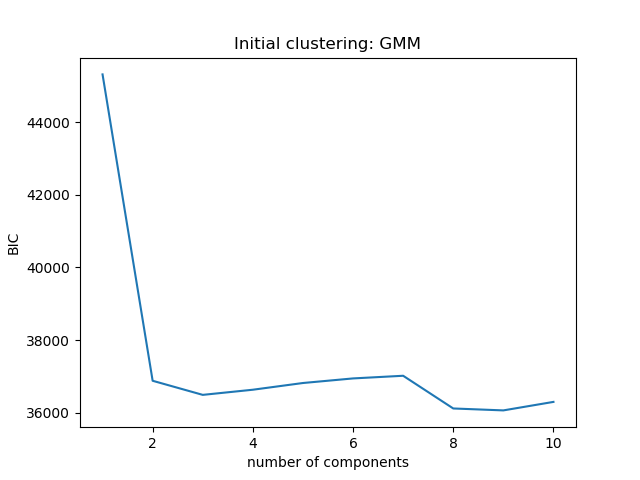
\includegraphics[width=8cm]{../pima/clustering1/gmm_init.png}
            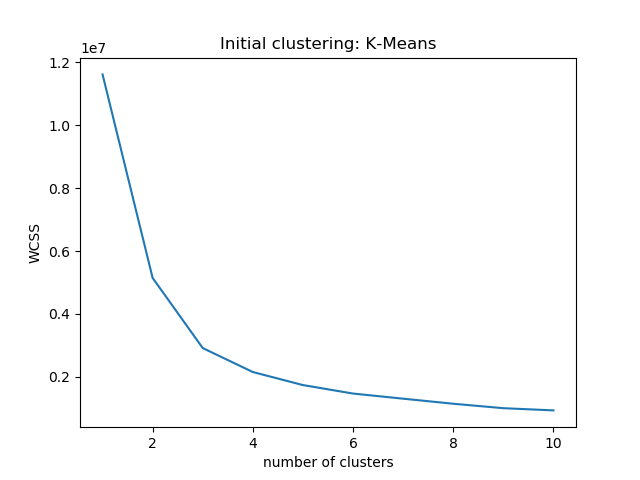
\includegraphics[width=8cm]{../pima/clustering1/km_init.png}

            In this dataset, a clear "elbow" can be seen at two clusters for the GMM,
            and there is a slight "elbow" at three clusters for the K-means. This problem
            is a binary classification problem (predicts whether someone has diabetes or not),
            so it is reasonable for the number of clusters to be close to two.

            \subsubsection{Initial clustering: Mushrooms dataset}

            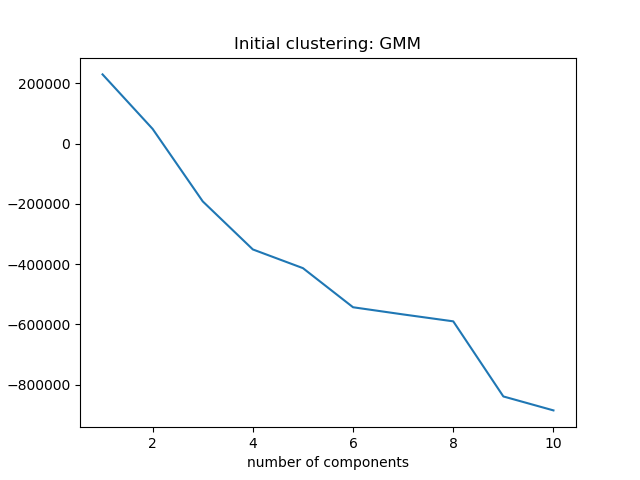
\includegraphics[width=8cm]{../mushrooms/clustering1/gmm_init.png}
            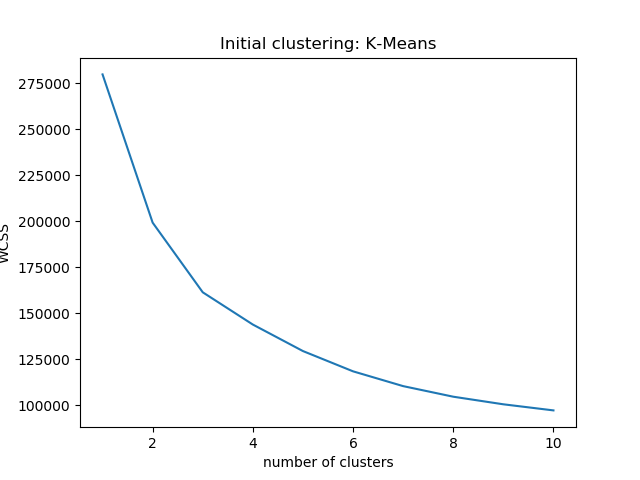
\includegraphics[width=8cm]{../mushrooms/clustering1/km_init.png}
            
            \subsection{PCA}

                PCA was run on a couple of the datasets. To make the datasets easy to visualize, the
                PCA was run such that the data was to be split into two components. Here are the
                results of the PCA that was performed:

            \subsubsection{PCA: Pima Indians Diabetes dataset}

            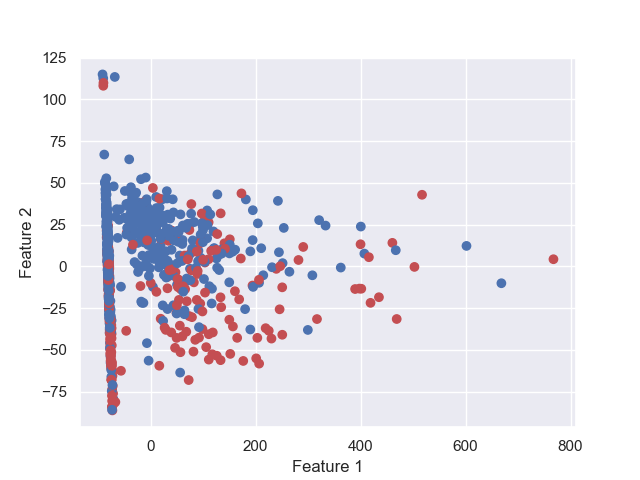
\includegraphics[width=8cm]{../pima/pca/diabetes_pca.png}

            \subsection{Clustering after PCA}

            The two datasets were clustered with the two algorithms
            after the PCA dimensionality reduction algorithms were run
            on them.

            \subsubsection{Clustering after PCA: Pima Indians Diabetes dataset}

            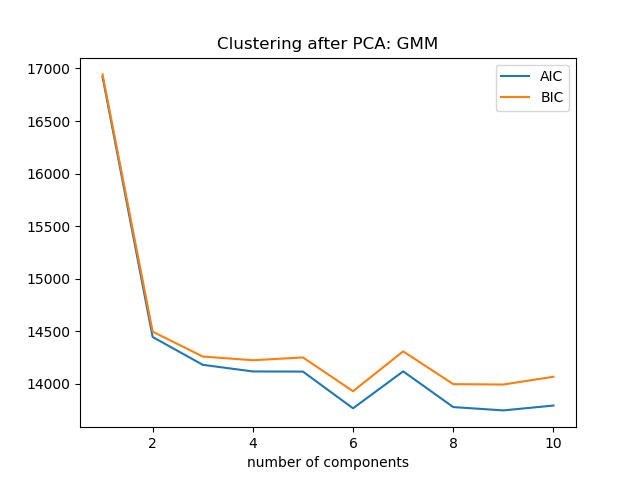
\includegraphics[width=8cm]{../pima/clustering2/gmm_pca.png}
            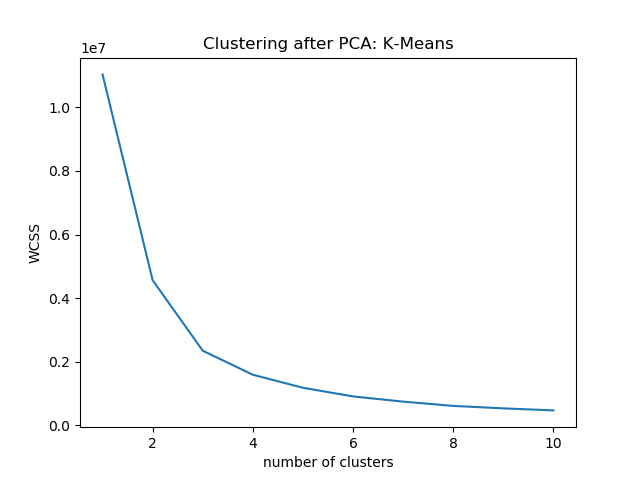
\includegraphics[width=8cm]{../pima/clustering2/km_pca.png}

            \subsection{Training a neural network after PCA}

            The Pima Indians dataset was split such that 60 percent of it
            was training data and 20 percent was testing data. Here is a plot
            of the accuracy of the neural network (training and testing) with
            respect to the number of principal components generated in the
            PCA algorithm:

            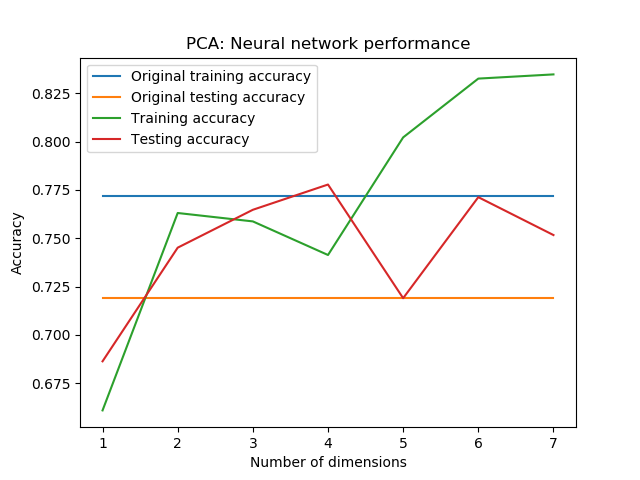
\includegraphics[width=8cm]{../pima/nn_pca/nn_pca.png}

            \subsection{Clustering for dimensionality reduction}

            The Pima Indians diabetes was split into a training and testing set (60
            percent training and 20 percent testing).

            Then, the GMM and the k-Means algorithm were each used to reduce the dimensions of
            the data for the Pima Indian Diabetes dataset. For each number of clusters,
            a neural network was trained to produce a mapping from the reduced data
            to labels. Here are the results for the training and testing
            accuracies:

            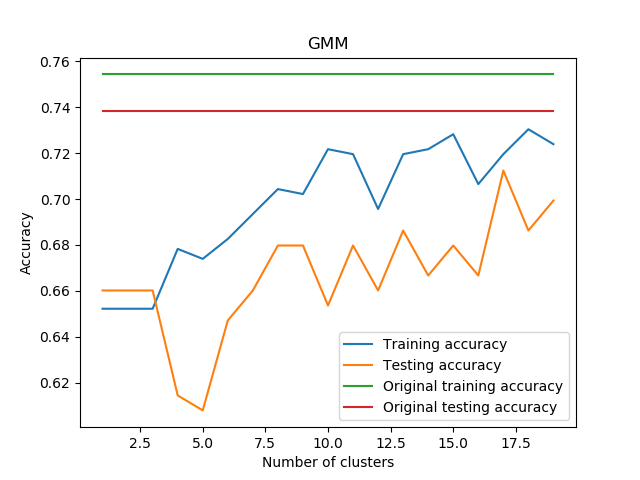
\includegraphics[width=8cm]{../pima/clustering3/gmm_acc.png}
            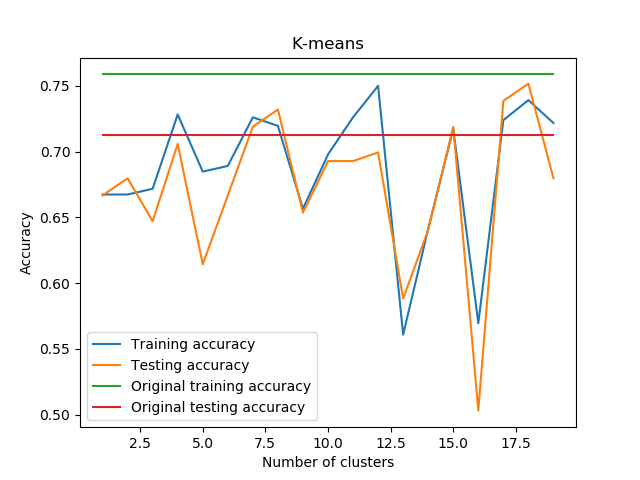
\includegraphics[width=8cm]{../pima/clustering3/km_acc.png}



        \section{Sources}

        [1] https://www.kaggle.com/uciml/pima-indians-diabetes-database



    \end{document}